\documentclass{article}
\usepackage[utf8]{inputenc}

\title{Baldwin-Barth turbulence model}
\author{El Namer Ayman }
\date{June 2020}
\usepackage[thinc]{esdiff}
\usepackage[euler]{textgreek}
\usepackage{graphicx}


\begin{document}

\maketitle

\section{Overview}
Baldwin-Barth is a one equation model, which was proposed in 1991 to close the RANS and Boussinesq hypothesis, the reasons that were stated for the suggestion of this model is that they have the goal to adequately predict several of the rubulent flow fields contained in the Viscous Transonic Airfoil Workshop. 
The model starts off with several steps that will start from a standard form of the k-epsilon equation, to which we will reach the final result, the applications of it and so on. This model, alongside with Spallart-Almaras, are one-equation models have been formulated after some time that presented silence in that regard. Those came after the Prandtl equation, which was the first one-equation RANS model. Whilist Baldwin-Barth and Spallart-Almaras are generalizations of the Nee-Kovasznay formulation.
The Baldwin-Barth model, can be denoted and divided in 2 parts B1 and B2, in which respectively, the first one, B1, studies it's originally specified (unmodified) freestream value of the eddy viscosity, while B2 uses a value of freestream velocity that satisfies a solution for the constant pressure boundary layer.
We will study the equations, BC, IC, auxiliary relations and so on, whereas we will try to define as accurately as possible all of the aspects of the Baldwin-Barth turbulence model.

\section{The equation, closure coefficients}

Here we can see that the model starts off with the RANS equation (1) and the Boussinesq hypothesis (2), at an attempt to be able to find from the equation: 

\begin{equation}
    \diffp{U_i}{t}+\diffp{U_iU_j}{{x_j}}=\frac{F_i}{\rho}-(\frac{1}{\rho})\diffp{P}{{x_i}}+\diffp{[(\nu+\nu_t)\diffp{U_i}{{x_j}}-\frac{2}{3}k\delta_{ij}]}{{x_j}}
\end{equation}

\begin{equation}
\tau_{ij}=\nu_t(\diffp{U_i}{{x_j}}+\diffp{U_j}{{x_i}})-\frac{2}{3}k\delta_{ij}
\end{equation}

\newpage

Now in these equations we need to define the Kinematic eddy viscosity (3), where we can define various values and coefficients.

\begin{equation}
    \nu_t={C_\mu}{\nu}{\widetilde{R}_t}{D_1}{D_2}
\end{equation}

The first term of the member, C{\textsubscript{\textmugreek}} is a closure coefficient, {\textnu} is the molecular viscosity, and the ${\widetilde{R}\textsubscript{t}}$ is the turbulence Reynolds number. From the latter value quantity, we can satisfy the equation (4), which will presente various closure coefficients and also auxiliar relations.


\begin{equation}
\diffp{(\nu{\widetilde{R}_t})}{t}+{U_j}\diffp{(\nu{\widetilde{R}_t})}{{x_j}}=({C_{\epsilon2}}{f_2}-{C_{\epsilon1}})\sqrt{{\widetilde{R}_t}{P}{\nu}}+({\nu}+\frac{\nu_t}{\sigma_\epsilon})\diffp{(\nu{\widetilde{R}_t})}{{x_j}{x_j}}-{\frac{1}{\sigma_\epsilon}}{\diffp{\nu_t}{{x_j}}}{\diffp{(\nu\widetilde{R}_t)}{{x_j}}}
    \end{equation}
    
    After defining the equation, we will be defining now the auxiliary equations and define the coefficients as it is shown in the following:

\bigskip
\bigskip
\begin{center}
    ${C_{\epsilon1}}=1,2$; ${C_{\epsilon_2}}=2,0$; ${C_\mu}=0,09$;
\end{center}
\bigskip
   \begin{center}
     ${A^+_2}=10$;
   ${A^+_0}=26$;
   \end{center}
\bigskip
      \begin{center}
   ${\kappa}=0,41$;
\end{center}
\bigskip
\begin{center}
    $\frac{1}{\sigma_\epsilon}=({C_{\epsilon1}}-{C_{\epsilon2}}){\frac{\sqrt{C_\mu}}{{\kappa}^2}}$
\end{center}
\bigskip
\begin{center}
    ${D_1}=1-{e}^{\frac{-y^+}{A_0^+}}$;
    ${D_2}=1-{e}^{\frac{-y^+}{A_2^+}}$
\end{center}
\bigskip
\begin{center}
    $P={\nu_t}[({\diffp{U_i}{{x_j}}}+{\diffp{U_j}{{x_i}}}){\diffp{U_i}{{x_j}}}-{\frac{2}{3}}{\diffp{U_k}{{x_k}}}{\diffp{U_k}{{x_k}}}$
\end{center}
\bigskip
\begin{center}
    ${f_2}={\frac{C_{\epsilon1}}{C_{\epsilon2}}}+({1-{\frac{C_{\epsilon2}}{C_{\epsilon1}}}})({\frac{1}{ky^+}}+{D_1}{D_2})[{\sqrt{{D_1}{D_2}}}+{\frac{y^+}{\sqrt{{D_1}{D_2}}}}({\frac{D_2}{A_0^+}}e^{\frac{-y^+}{A_0^+}}+{\frac{D_2}{A_2^+}}e^{\frac{-y^+}{A_2^+}})]$
\end{center}
\bigskip
\newpage
And here we can see that the first three rows present the closure coefficients, regarding C, $A^+$ and \textkappa, while the other values present the auxiliary equations needed to solve the Baldwin-Barth equation.
The equation doesn't present as for now an accurate value of the Turbulent Kinetic energy, but Baldwin-Barth still present an approximate equation (5) which defines it, where, though, we need to define the Production value (6) of the turbulent kinetic energy, which we had previously shown, anyways above as P, in order to calculate the K value, as we can see from the following equations.

\begin{equation}
    {k^2}={\nu}{\widetilde{R}_t}{P}
\end{equation}
\begin{equation}
    {P}={\nu_t}({\diffp{U_i}{{x_j}}}+{\diffp{U_j}{{x_i}}}){\diffp{U_i}{{x_j}}}-{\frac{2}{3}}{\nu_t}({\diffp{U_k}{{x_k}}})^2
\end{equation}

\section{Reccomended boundary, limitations}
As we have introduced, the reasoning to the definition of this model is the inability of algebraic models to accurately predict turbulent phenomena in multiple scaled layers. They deduced their model, in fact, was deduced based on the non-linear combination of the $k$-$\epsilon$ equation. The model solves the $\widetilde{R}_t$ which is related to the eddy viscosity ${\nu_t}$. Incompressible flow over a flat plate with zero pressure gradient is used to determine suitable damping functions and to calibrate the model. The objective of this model, as we can deduce, is similar to Spallart-Almaras, hence the prediction of the turbulence fenomena in shear flows with one equation. A difference we can say is that SA was derived independent of a two-equation model, giving it more freedom than BB, and SA is independent from the value $y^+$, and has a built in transition term which showcases relatively smoothly a transition of the flow to turbulent.
The boundary conditions are pretty much defined as same treatment as working variables in both SA and BB, which we will showcase just below.

\bigskip
\begin{center}
Viscous wall: ${\widetilde{R}_t}=0$
\end{center}
\bigskip
\begin{center}
    Inviscid wall, Outflow: ${\widetilde{R}_{tb}}={\widetilde{R}_{ta}}$
\end{center}
\bigskip
\begin{center}
    Singular axis: ${\widetilde{R}_{tb}}={AVG}{\widetilde{R}_{ta}})$
\end{center}
\bigskip
\begin{center}
    Inflow: ${\widetilde{R}_{t}}={\widetilde{R}_{t}}{\infty}=0.1$
\end{center}
\bigskip
\begin{center}
    Self closing: ${\widetilde{R}_{tb}}={0.5}({\widetilde{R}_{t2}}+{{\widetilde{R}_{t(max-1)}}})$
\end{center}
\bigskip
A denotes the adjacent grid point while B denotes the boundary grid point.

\newpage
Several test cases were used to validate the BB model (as long as the SA) along with 2-equation models and so on, in various cases which we may discuss in as the following:
\subsection{Flat Plate}
The flat plate analyzed was at free stream conditions with M=4.54, P=0.19 psi and T=110 R. The results dont show much difference between BB and the most of other 1-equation and 2-equation models, concluding that they are very well comparable, with exception of skin friction coefficient. Baldwin is shown with a straight line, the other lines are other turbulence models
\begin{center}
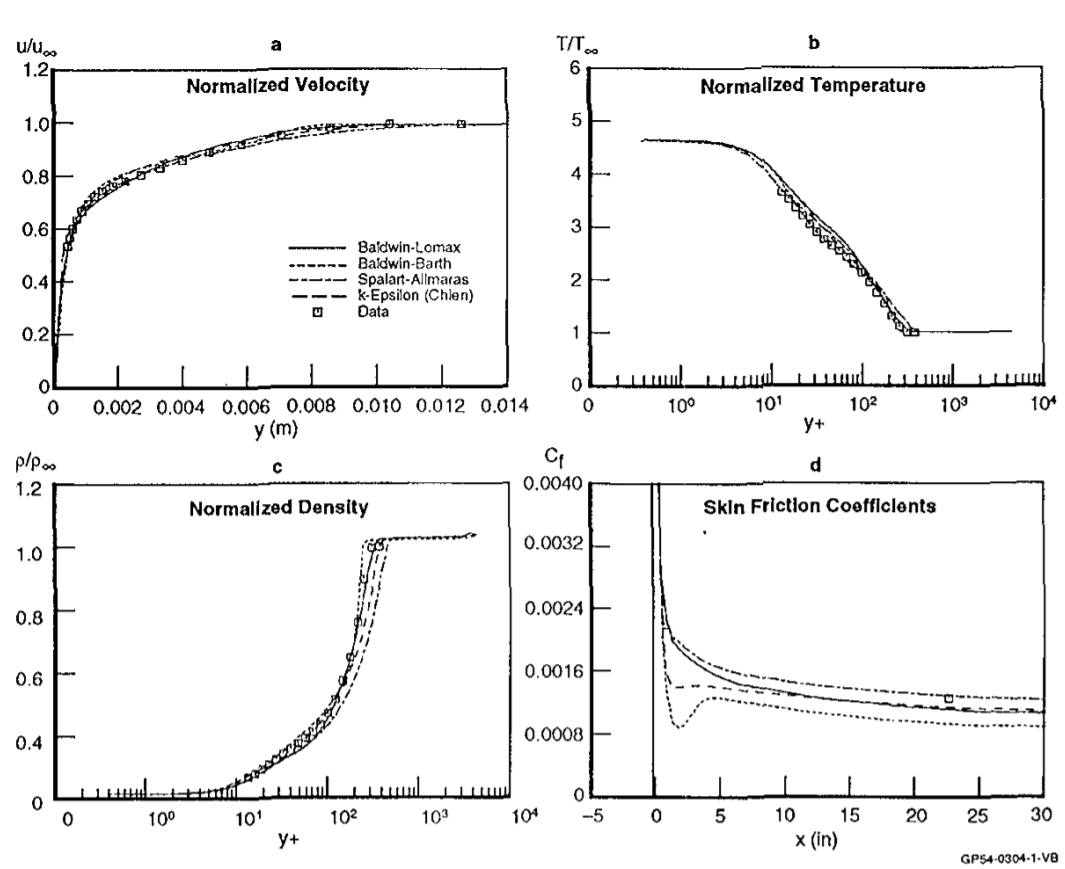
\includegraphics[scale=0.5]{Graph1.PNG}
\end{center}
\newpage
\subsection{Single element airfoil}
Our second and last example we will use is the single element airfoil for comparison of the various models, in particular the RAE-2822 airfoil where we impose as initial conditions the velocity, temperature and pressure yet again, in the initial condition of free flow stream. The models of one-equation are quite comparable within one another as it is showcased, yet, none of the models, included BB, did not predict the suction peak at the leading edge of the airfoil. Baldwin-Barth definitely shows itself having the best results at the upstream of the shock, while the other one-equation models, like SA; tend to overpredict that range the friction levels, compared to the experimental data.
So the BB is more consistent in terms of skin friction, compared to the others that show more accuracy after the shock. Yet again, the Baldwin-Barth result is the outlined case, while the others are dashed, clearly showcased the difference in the friction coefficient, being clearly lower in the most of the area than the other cases.
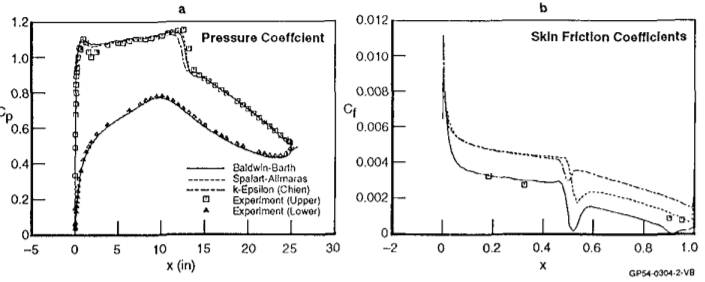
\includegraphics[scale=0.8]{Graph2.PNG}

\section{Conclusion}
We can see that the Baldwin-Barth model showcased improvements compared to the standard Baldwin-Lomax which is an algebraic model. So the upside is more accuracy and efficiency, while one of the downsides is the requirement of 15\% more CPU node per iteration compared to B-L mode. However, the total CPU to obtain a converged solution is less for the 1-equation models than Baldwin-Lomax thanks to the smooth and continuous turbulent distribution that we obtain.

So, the one-equation are significantly more robust and efficient, and not require the degree of grid packing near wall boundaries that the two-equation require.
The differences of precision, except for a few cases, have not been very different, except for a detailed analysis of a shear layer where BB falls flat, as it predicts worse than the 2-eq model, in particular the Chien model.
Furthermore, compared to the two equation model, BB has the drawback of representing properly the two scales that are required to build the eddy viscosity.
\newpage
\begin{thebibliography}{}

\bibitem{}Vijay A. Sai and Frederick M. Lutfy (2012), Analysis of the Baldwin-Barth and Spalart-Allmaras one-equation turbulence model.

\bibitem{} Baldwin, B.S. and Barth, T.J. (1990), A One-Equation Turbulence Transport Model for High Reynolds Number Wall-Bounded Flows, NASA TM 102847.
\bibitem{}  M. Mani, P. Willhite, J. Ladd McDonnell Douglas Corporation, St. Louis, Missouri (1995), Performance of One-Equation Turbulence Models .in CFD Applications.
\end{thebibliography}

\end{document}